% !TEX encoding = UTF-8 Unicode
% -*- coding: UTF-8; -*-
% vim: set fenc=utf-8
\section{Ход работы}
    
    Данная лабораторная работа выполняется на виртуальной машине с ОС Windows server 2008 R2 с установленной службой активных каталогов Active Directory.\par
    Для запуска диспетчера сервера (рисунок \ref{img:02}) выполним команду <<servermanager.msc>> через диалоговое окно <<Выполнить>> (рисунок \ref{img:01}).\par
    
	\begin{figure}[h!]
        \centering
        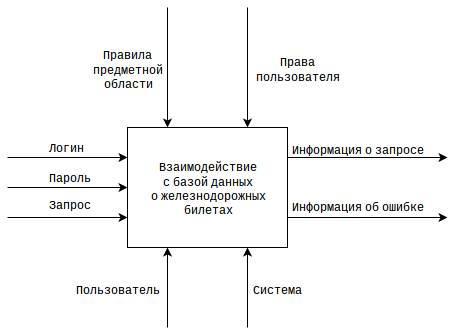
\includegraphics[width=0.7\textwidth]{1}
        \caption{Запуск диспетчера сервера}
        \label{img:01}
    \end{figure}
    
    \begin{figure}[h!]
        \centering
        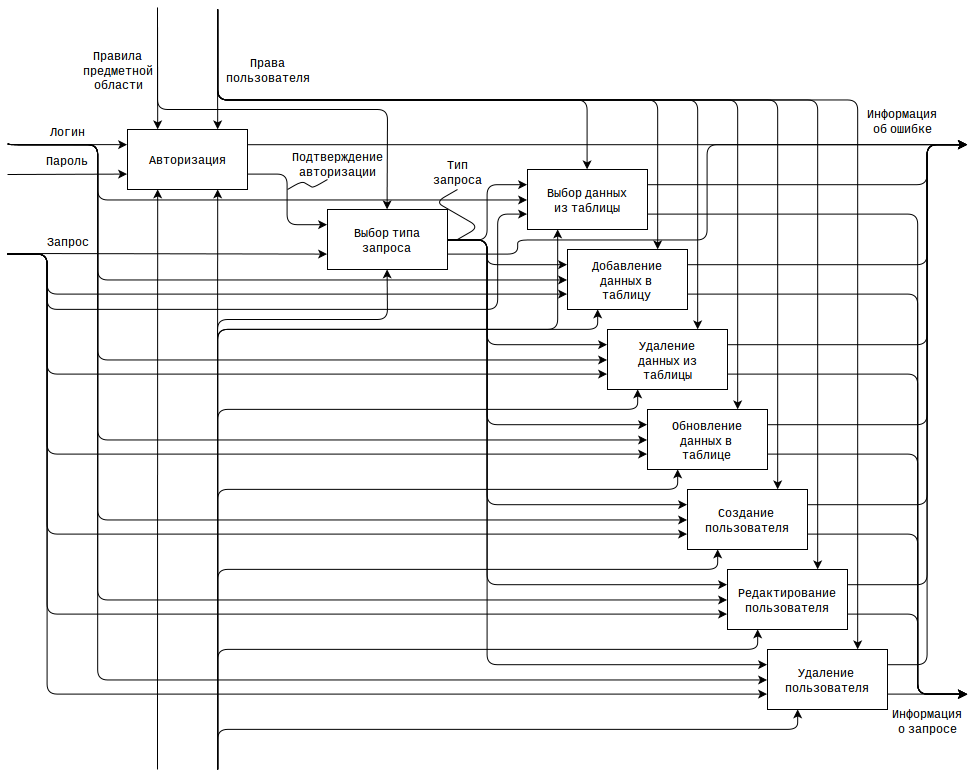
\includegraphics[width=0.7\textwidth]{2}
        \caption{Диспетчер сервера}
        \label{img:02}
    \end{figure}
    
    Затем нажмем <<ДОБАВИТЬ РОЛИ>>. В открывшемся окне отметим пункт <<СЛУЖБЫ СЕРТИФИКАЦИИ ACTIVE DIRECTORY>> (рисунок \ref{img:03}).\par
    
    \clearpage

    \begin{figure}[h!]
        \centering
        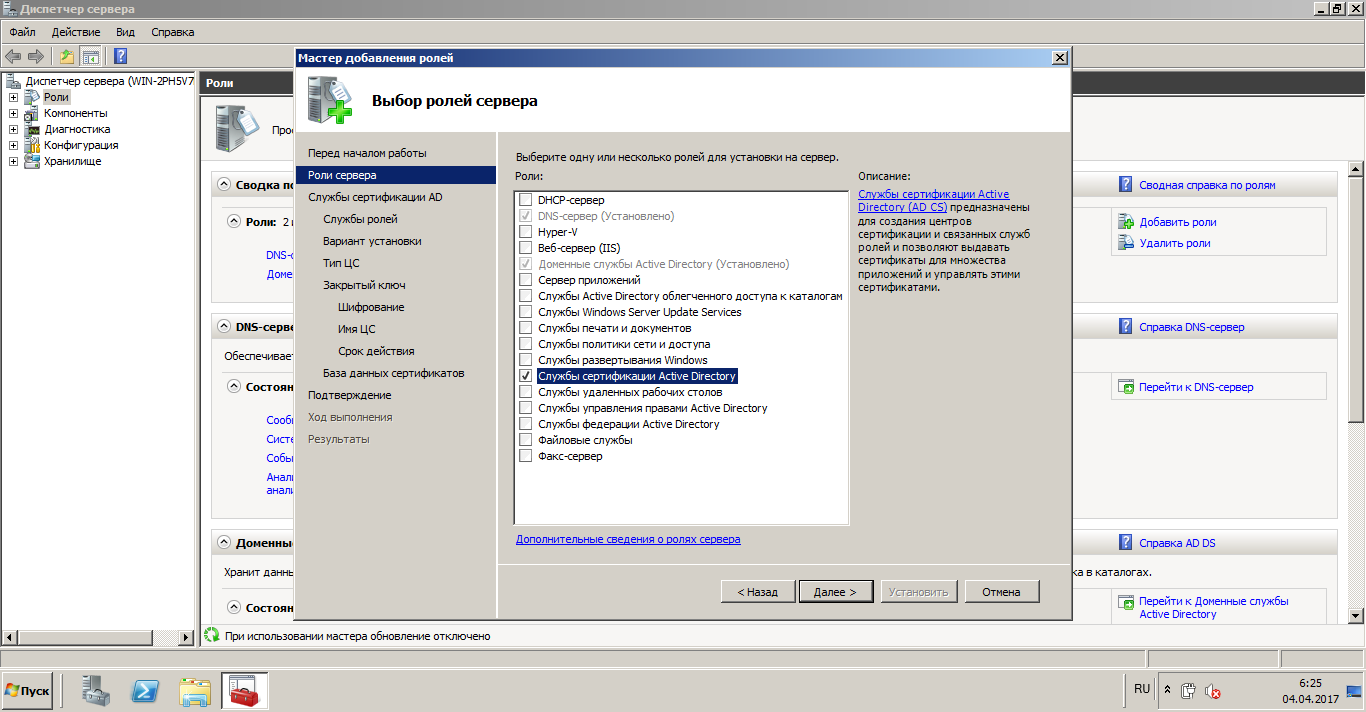
\includegraphics[width=0.7\textwidth]{3}
        \caption{Добавление ролей служб сертификации Active Directory}
        \label{img:03}
    \end{figure}
    
    Поставим галочки напротив служб <<ЦЕНТР СЕРТИФИКАЦИИ>> и <<СЛУЖБА РЕГИСТРАЦИИ В ЦЕНТРЕ СЕРТИФИКАЦИИ ЧЕРЕЗ ИНТЕРНЕТ>> (рисунок \ref{img:04}).\par
    
    \begin{figure}[h!]
        \centering
        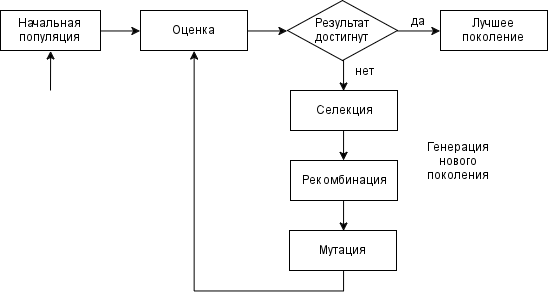
\includegraphics[width=0.7\textwidth]{4}
        \caption{Выбор служб ролей}
        \label{img:04}
    \end{figure}
    
    В задании типа установки выберем <<ПРЕДПРИЯТИЕ>> (рисунок \ref{img:05}).\par
    
    \begin{figure}[h!]
        \centering
        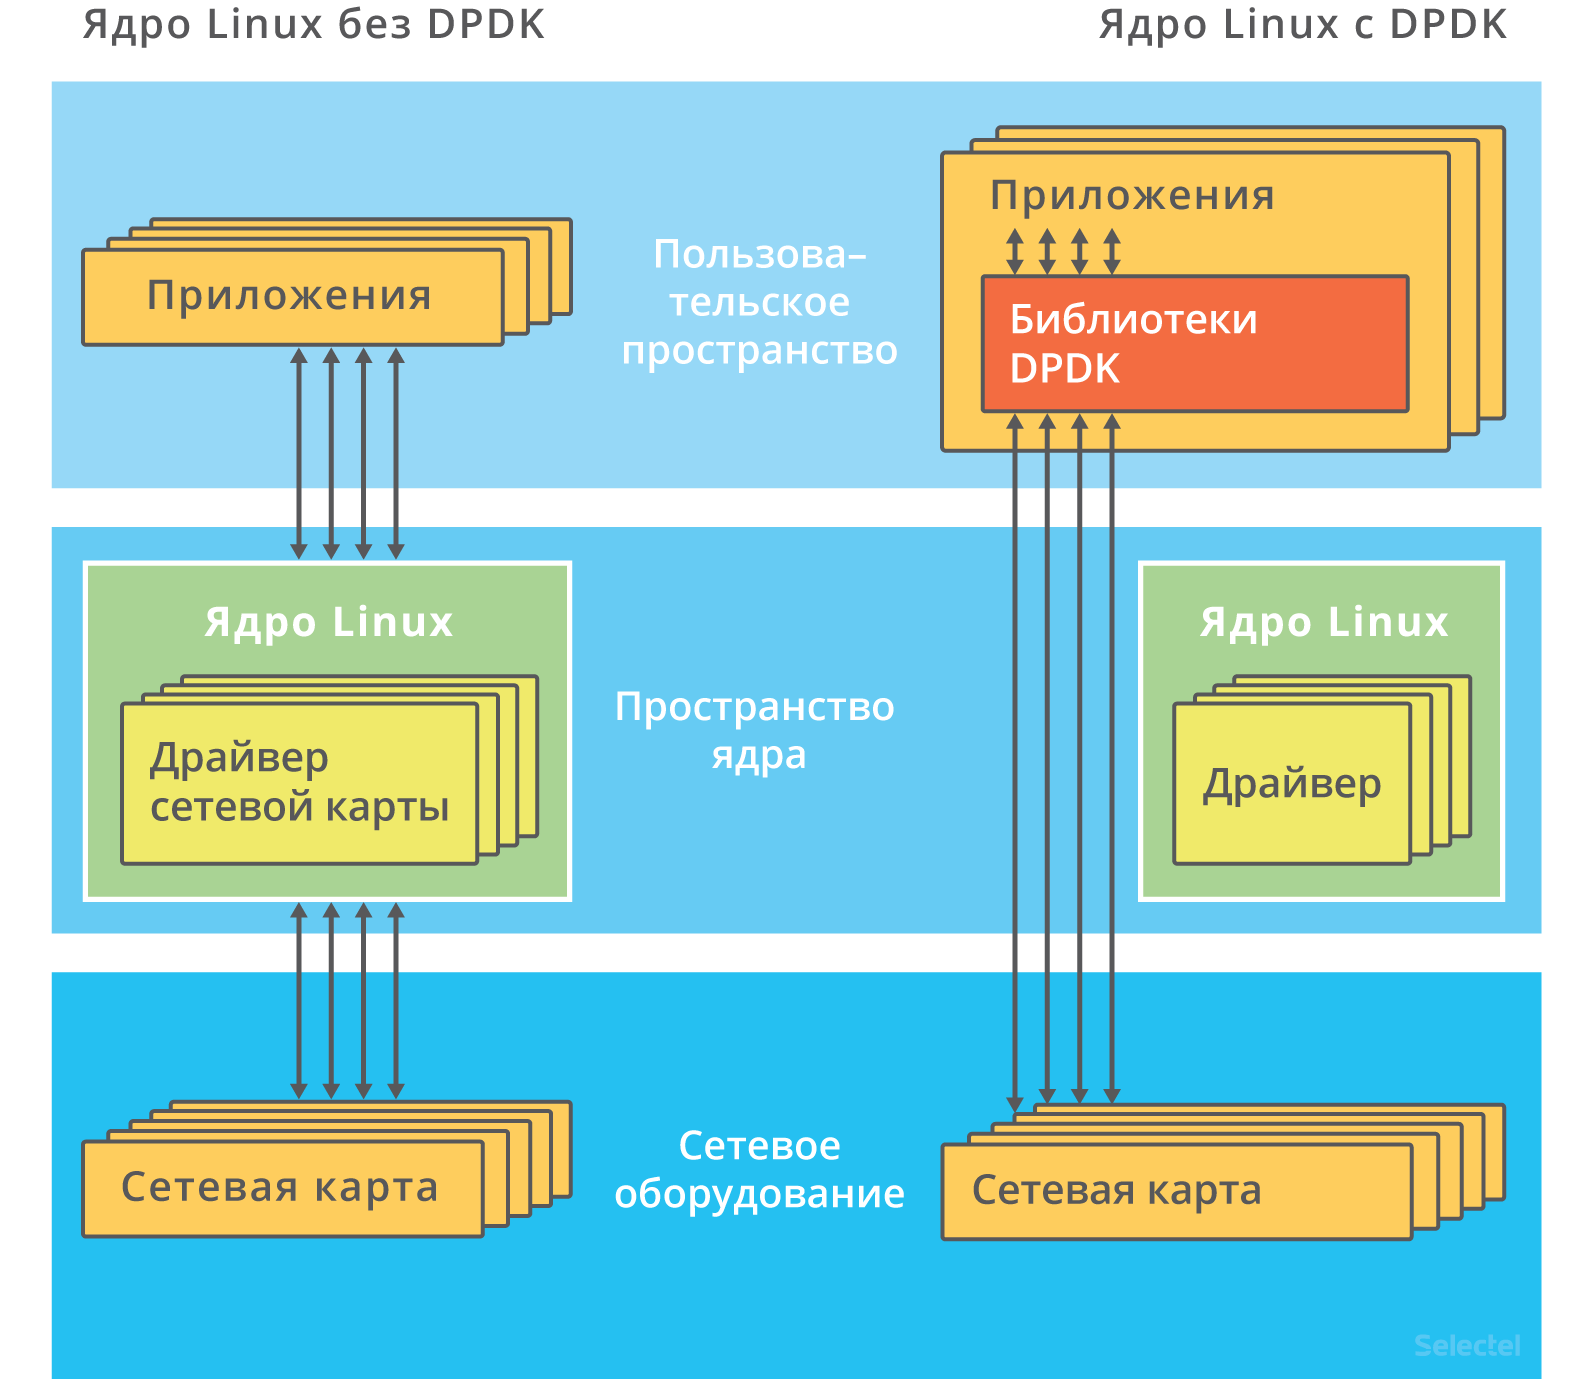
\includegraphics[width=0.7\textwidth]{5}
        \caption{Задание типа установки}
        \label{img:05}
    \end{figure}
    
    При задании типа ЦС выберем <<КОРНЕВОЙ ЦС>> (рисунок \ref{img:06}).\par
    
    \begin{figure}[h!]
        \centering
        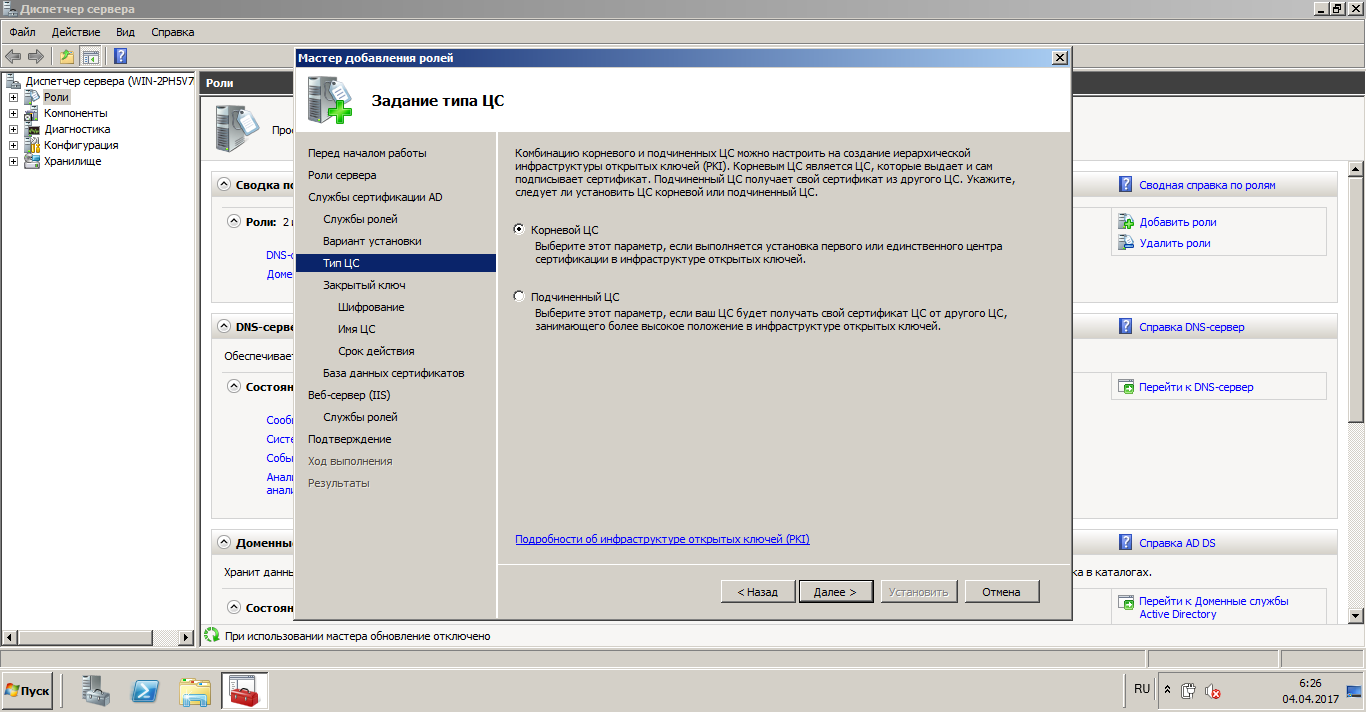
\includegraphics[width=0.7\textwidth]{6}
        \caption{Задание типа центра сертификации}
        \label{img:06}
    \end{figure}
    
    Далее выберем пункт <<СОЗДАТЬ НОВЫЙ ЗАКРЫТЫЙ КЛЮЧ>> (рисунок \ref{img:07}).\par

    \begin{figure}[h!]
        \centering
        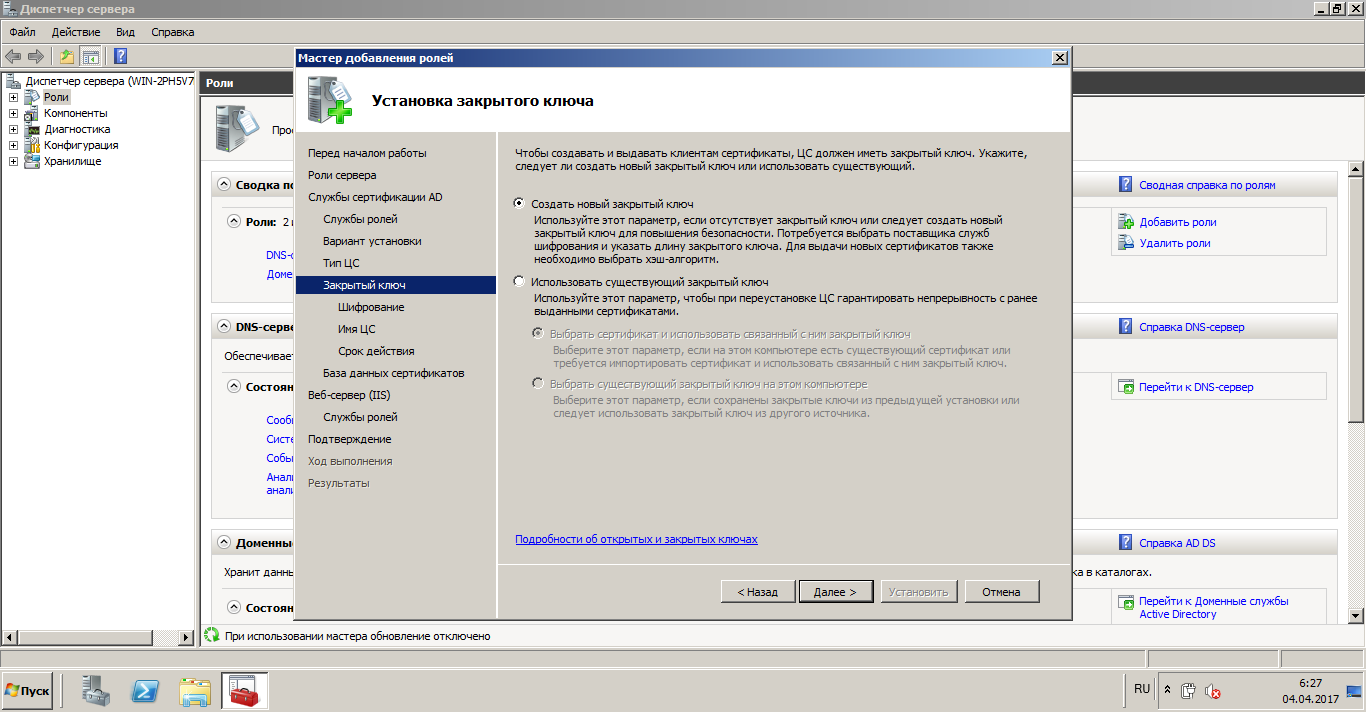
\includegraphics[width=0.7\textwidth]{7}
        \caption{Установка закрытого ключа}
        \label{img:07}
    \end{figure}
    